\documentclass[compress, blue]{beamer}
\mode<presentation>
\usetheme{Warsaw}
%\usetheme{Hannover}
%\usecolortheme{lily}
\useoutertheme[subsection=false]{smoothbars}
%\useinnertheme{rectangles}
%\hypersetup{pdfpagemode=FullScreen} % makes your presentation go automatically to full screen
\setbeamertemplate{footline}[text line]{} % makes the footer EMPTY

%\usetheme{Hannover}
%\usetheme{default}
\definecolor{links}{HTML}{2A1B81}
\hypersetup{colorlinks,linkcolor=,urlcolor=links}
\usepackage{listings}
\usepackage{wrapfig}
\usepackage{mdwlist}
\usepackage{subfigure}
\usepackage[normalem]{ulem}

\newcommand{\RR}{\mathbb{R}}
\newcommand{\pair}[2]{
\begin{columns}
\column{.5\textwidth}
{#1}
\column{.5\textwidth}
{#2}
\end{columns}}


\lstset{ 
  basicstyle=\scriptsize,           % the size of the fonts that are used for the code
%  numbers=left,                   % where to put the line-numbers
%  numberstyle=\tiny\color{gray},  % the style that is used for the line-numbers
%  stepnumber=2,                   % the step between two line-numbers. If it's 1, each line 
                                  % will be numbered
%  numbersep=5pt,                  % how far the line-numbers are from the code
  backgroundcolor=\color{white},      % choose the background color. You must add \usepackage{color}
  showspaces=false,               % show spaces adding particular underscores
  showstringspaces=false,         % underline spaces within strings
  showtabs=false,                 % show tabs within strings adding particular underscores
%  frame=single,                   % adds a frame around the code
  rulecolor=\color{black},        % if not set, the frame-color may be changed on line-breaks within not-black text (e.g. commens (green here))
  tabsize=2,                      % sets default tabsize to 2 spaces
  captionpos=b,                   % sets the caption-position to bottom
  breaklines=true,                % sets automatic line breaking
  breakatwhitespace=false,        % sets if automatic breaks should only happen at whitespace
  title=\lstname,                   % show the filename of files included with \lstinputlisting;
                                  % also try caption instead of title
  keywordstyle=\color{blue},          % keyword style
  commentstyle=\color{dkgreen},       % comment style
  stringstyle=\color{mauve},         % string literal style
  escapeinside={\%*}{*)},            % if you want to add LaTeX within your code
  morekeywords={*,...}               % if you want to add more keywords to the set
}



\begin{document}
\title{SymPy.stats: Uncertainty Modeling}
\author{Matthew Rocklin}
\date{July, 2012}
\institute{University of Chicago}

\begin{frame}
\maketitle
\end{frame}

\section{Introduction}
\subsection{I}

\begin{frame}{Topics}
    \begin{itemize}
        \item Uncertainty
        \item Modeling
        \item Symbolics
        \item Multi-Compilation
    \end{itemize}
\end{frame}

\begin{frame}{Data-Driven Statistics vs. Uncertainty Modeling}

\begin{columns}
    \column{.5\textwidth}
    Last Talk - Pandas:
    \indent Data Analysis
    \begin{figure}
        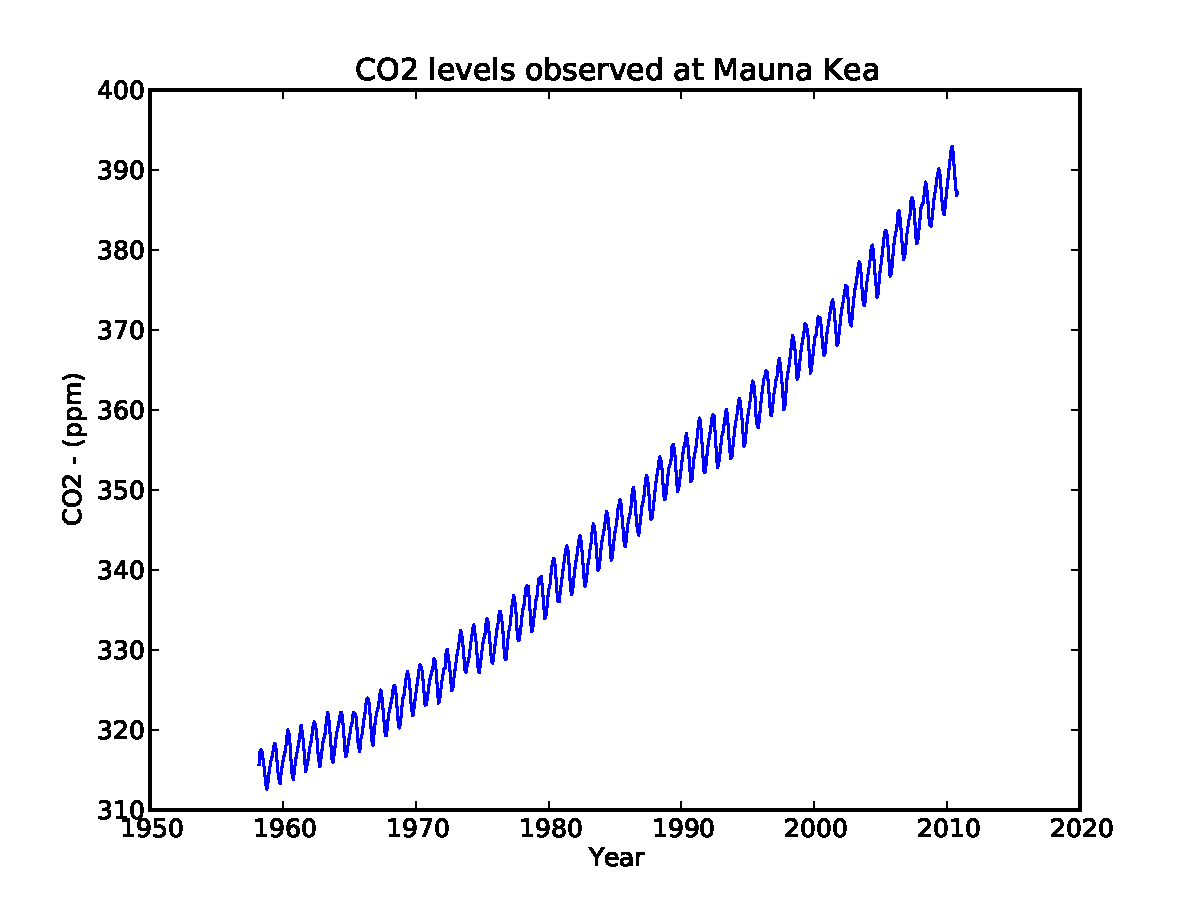
\includegraphics[width=\textwidth]{images/mauna-kea-co2.pdf}
        \caption{Historical CO2 Data from Mauna Kea observatory}
    \end{figure}
    \column{.5\textwidth}
    This Talk - SymPy.Stats
    \indent Mathematical Modeling with Uncertainty
    \begin{figure}
        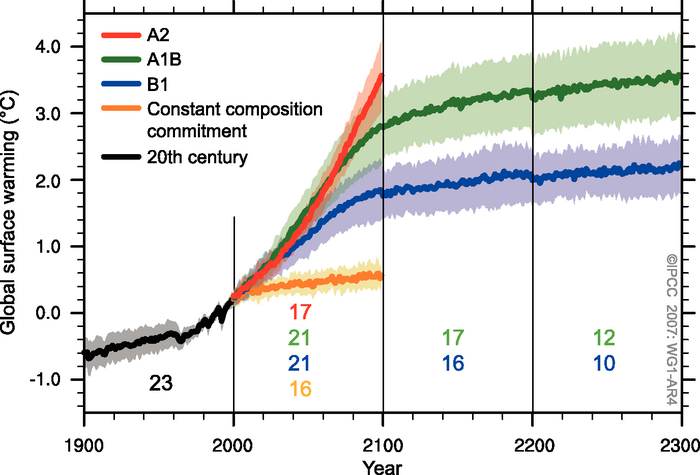
\includegraphics[width=\textwidth]{images/figure-ts-32-l.png}
        \caption{CO2 Predictions with uncertainty bounds}
    \end{figure}
\end{columns}
\end{frame}

\begin{frame}{Uncertainty }
\begin{columns}

\column{.25\textwidth}
\begin{figure}[ht]
\includegraphics[width=\textwidth]{images/wind}
\end{figure}
Windspeed \\30 km/hr
\pause
\column{.25\textwidth}
\begin{figure}[ht]
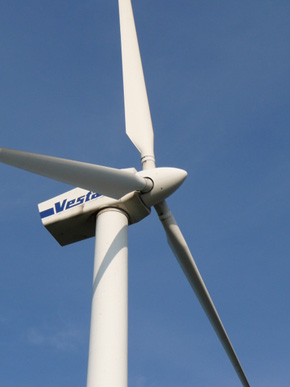
\includegraphics[width=\textwidth]{images/windmill}
\end{figure}
Wind Power \\ 50 KW

\pause
\column{.25\textwidth}
\begin{figure}[ht]
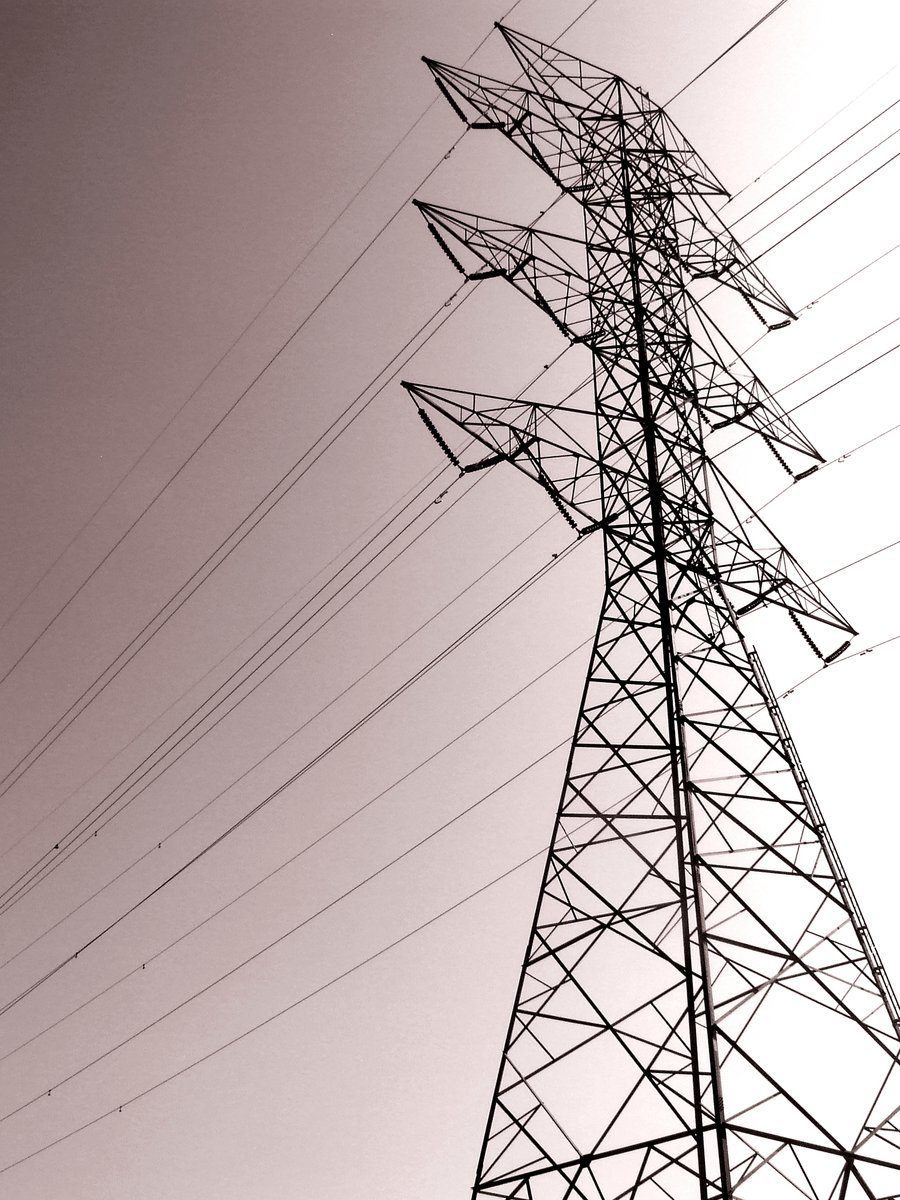
\includegraphics[width=\textwidth]{images/electricity}
\end{figure}
Electricity \\ 40 KW

\pause
\column{.25\textwidth}
\begin{figure}[ht]
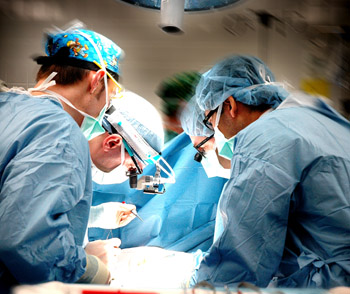
\includegraphics[width=\textwidth]{images/surgery}
\end{figure}
Lights are on!

\end{columns}
\end{frame}


\begin{frame}{Uncertainty }
Measurements are Distributions, not Scalars

\begin{columns}

\column{.25\textwidth}
\begin{figure}[ht]
\includegraphics[width=\textwidth]{images/wind}
\end{figure}
WindSpeed:
Around 30 km/hr
\begin{figure}[ht]
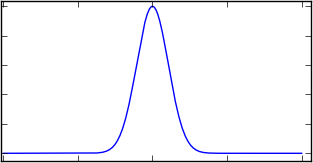
\includegraphics[width=\textwidth]{images/normal}
\end{figure}

\column{.25\textwidth}
\begin{figure}[ht]
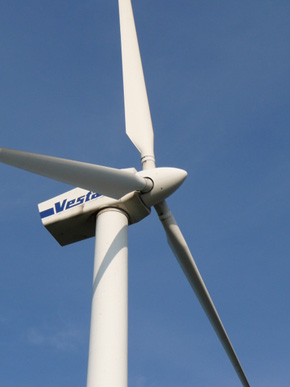
\includegraphics[width=\textwidth]{images/windmill}
\end{figure}
WindPower:
\begin{figure}[ht]
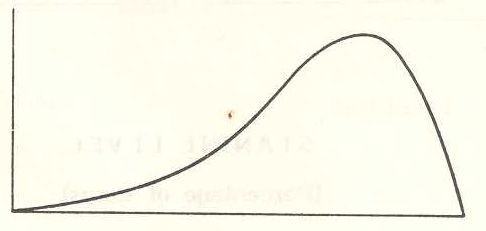
\includegraphics[width=\textwidth]{images/skew}
\end{figure}

\column{.25\textwidth}
\begin{figure}[ht]
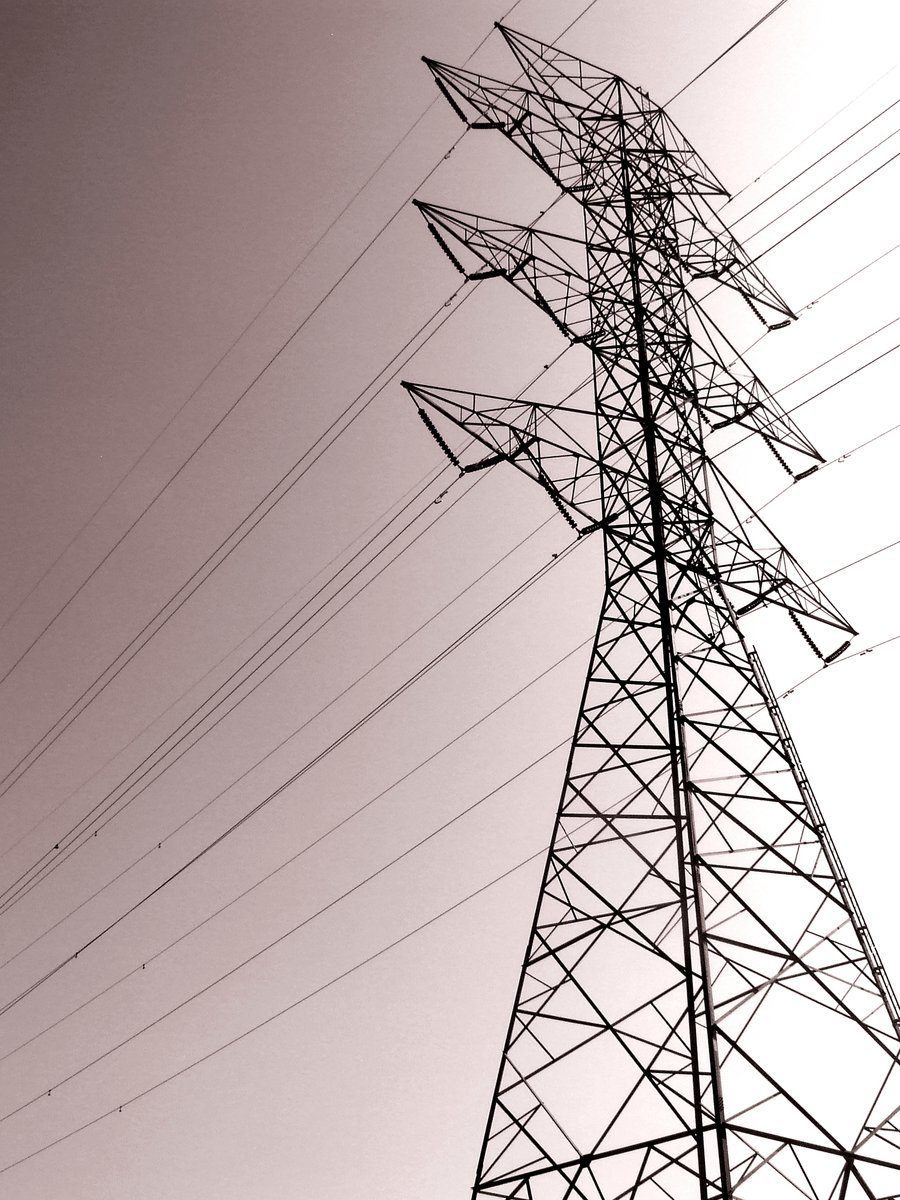
\includegraphics[width=\textwidth]{images/electricity}
\end{figure}
Electricity:
\begin{figure}[ht]
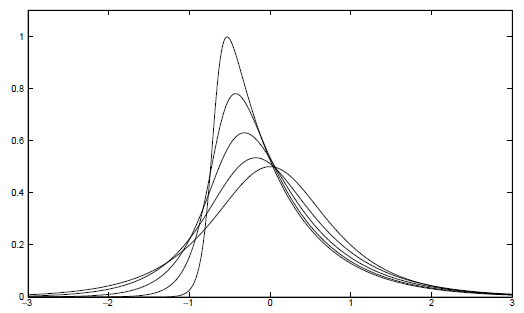
\includegraphics[width=\textwidth]{images/skew2}
\end{figure}

\column{.25\textwidth}
\begin{figure}[ht]
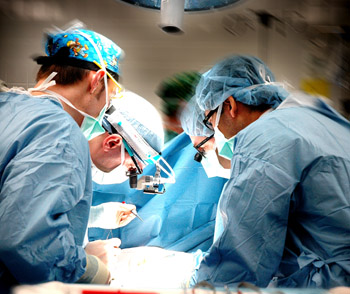
\includegraphics[width=\textwidth]{images/surgery}
\end{figure}
Lights stay on?

\end{columns}

\end{frame}


\section{Modeling}
\subsection{I}
\begin{frame}[semiverbatim, fragile]{Kinematics - Direct Solution}
\begin{columns}
    \column{.5\textwidth}<2->

\begin{lstlisting}
# Define inputs
x0 = 0
y0 = 0
yf = -30 # target height 
g = -10 # gravity 
v = 30 # m/s
theta = pi/4

# Solve 
while(y > yf):
    t+=dt
    y = y0 + v*sin(theta)*t 
           + g*t**2 / 2
}

x = x0 + v*cos(theta)*t
\end{lstlisting}

    \column{.5\textwidth}<1->
    \begin{figure}
        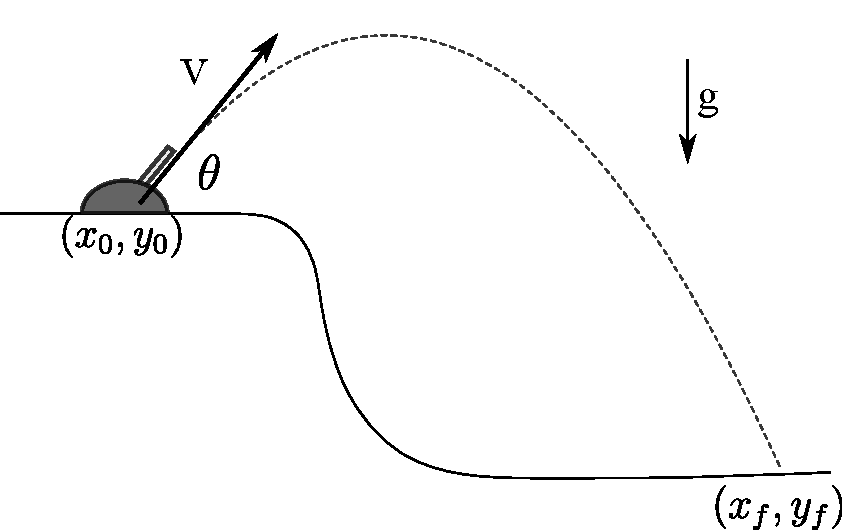
\includegraphics[width=\textwidth]{images/cannon.pdf}
    \end{figure}
\end{columns}
\end{frame}


% Combines statement of the problem with the method of solution

\begin{frame}[semiverbatim, fragile]{Kinematics - Modeling}
\begin{columns}
    \column{.5\textwidth}

\begin{lstlisting}
# Define inputs
x0 = 0
y0 = 0
yf = -30 # target height 
g = -10 # gravity 
v = 30 # m/s
theta = pi/4

# Define Model
t = Symbol('t') 
x = x0 + v*cos(theta)*t
y = y0 + v*sin(theta)*t 
       + g*t**2 / 2
impact_time = solve(y - yf, t)
xf = x0 + v*cos(theta)*impact_time

\end{lstlisting}

    \column{.5\textwidth}
    \begin{figure}
        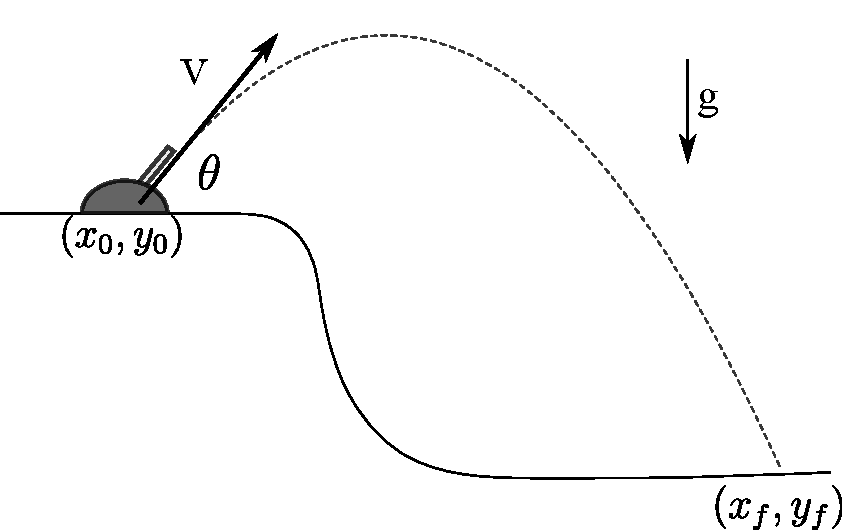
\includegraphics[width=\textwidth]{images/cannon.pdf}
    \end{figure}
\end{columns}
\end{frame}

\begin{frame}[semiverbatim, fragile]{Kinematics - Full SymPy}
\begin{columns}
    \column{.5\textwidth}

\begin{lstlisting}
# Define inputs
x0 = Symbol('x_0')
y0 = Symbol('y_0') 
yf = Symbol('y_f')
g = Symbol('g')
v = Symbol('v')
theta = Symbol('theta')

# Define Model
t = Symbol('t') 
x = x0 + v*cos(theta)*t
y = y0 + v*sin(theta)*t 
       + g*t**2 / 2
impact_time = solve(y - yf, t)
xf = x0 + v*cos(theta)*impact_time

\end{lstlisting}

%\begin{eqnarray*}
%impact time = \frac{- v \sin{\left(\theta \right)} + \sqrt{- 4 g y_{0} + 4 g
%y_f + v^{2} \sin^{2}{\left(\theta \right)}}}{2 g}  \\
%x_f  =  x_{0} + \frac{v \left(- v \sin{\left(\theta \right)} + \sqrt{- 4 g y_{0} + 4 g y_f + v^{2} \sin^{2}{\left(\theta \right)}}\right) \cos{\left(\theta \right)}}{2 g}
%\end{eqnarray*}
    \column{.5\textwidth}
    \begin{figure}
        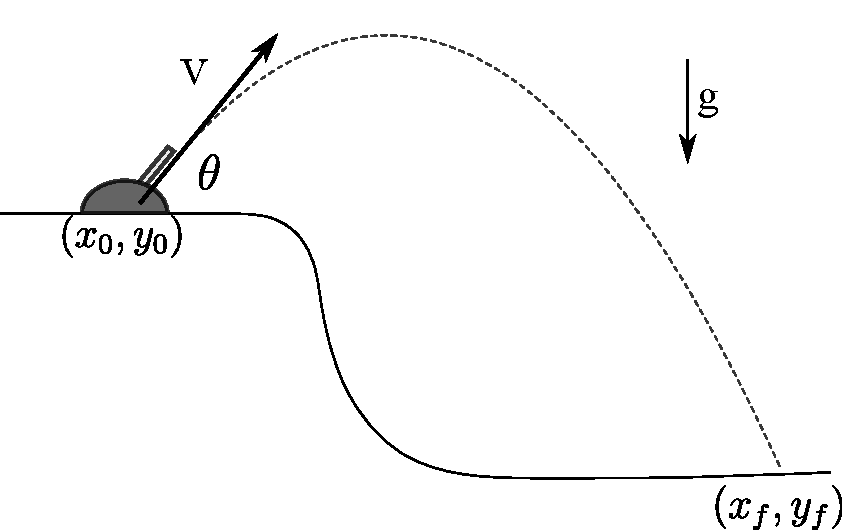
\includegraphics[width=\textwidth]{images/cannon.pdf}
    \end{figure}
\end{columns}
\end{frame}

\begin{frame}{Kinematics - Graph}
    SymPy generates a graph
    \begin{figure}
        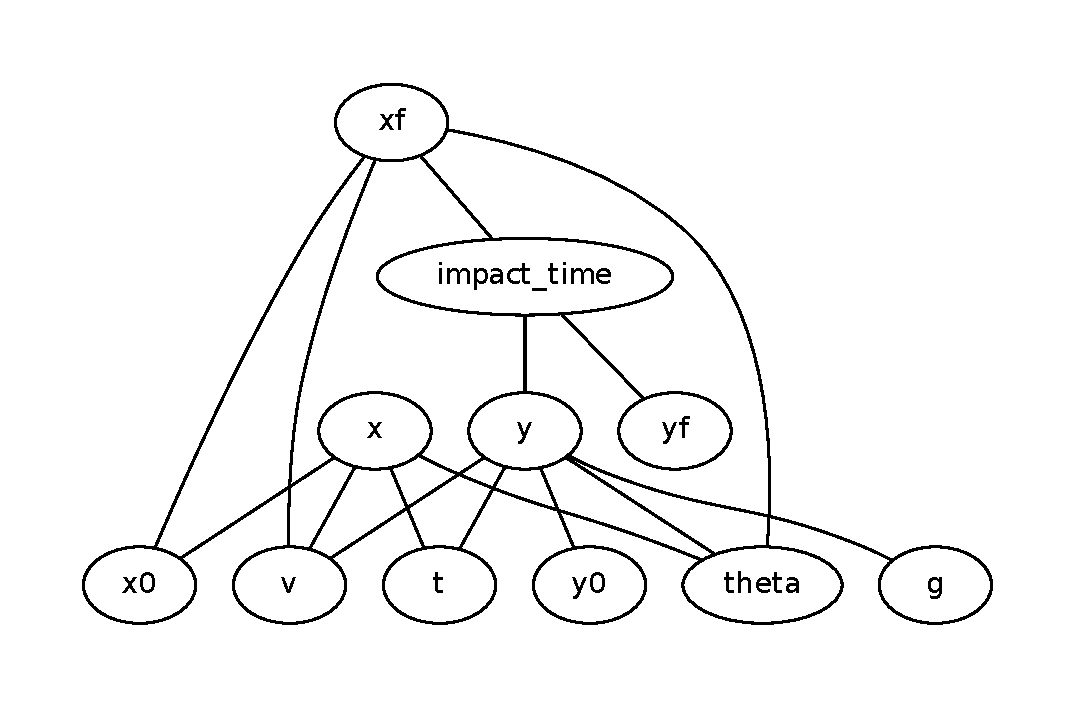
\includegraphics[width=\textwidth]{images/dag.pdf}
    \end{figure}
\end{frame}

\begin{frame}{Kinematics - Computing on a Graph}
\begin{eqnarray*}
    \textrm{impact time} & = & \frac{- v \sin{\left(\theta \right)} 
            + \sqrt{- 4 g y_{0} + 4 g y_f + v^{2} 
            \sin^{2}{\left(\theta \right)}}}{2 g}  \\
    x_f & = & x_{0} + \frac{v \left(- v \sin{\left(\theta \right)} 
            + \sqrt{- 4 g y_{0} + 4 g y_f + v^{2} 
            \sin^{2}{\left(\theta \right)}}\right) 
             \cos{\left(\theta \right)}}{2 g}
\end{eqnarray*}
\end{frame}

\section{Uncertainty}
\subsection{I}
\begin{frame}[semiverbatim, fragile]{Random Variables}
Introducting SymPy.stats
\begin{columns}<1->
    \column{.5\textwidth}


\begin{lstlisting}
>>> from sympy.stats import *
>>> # v = Symbol('v')
>>> v = Normal('v', 30, 1)

>>> # Plot the density
>>> pdf = density(v)
>>> plot(pdf(z), (z, 27, 33))
\end{lstlisting}
$$\frac{\sqrt{2} e^{- \frac{1}{2} \left(z -30\right)^{2}}}{2 \sqrt{\pi}}
$$
    \column{.5\textwidth}
    \begin{figure}
        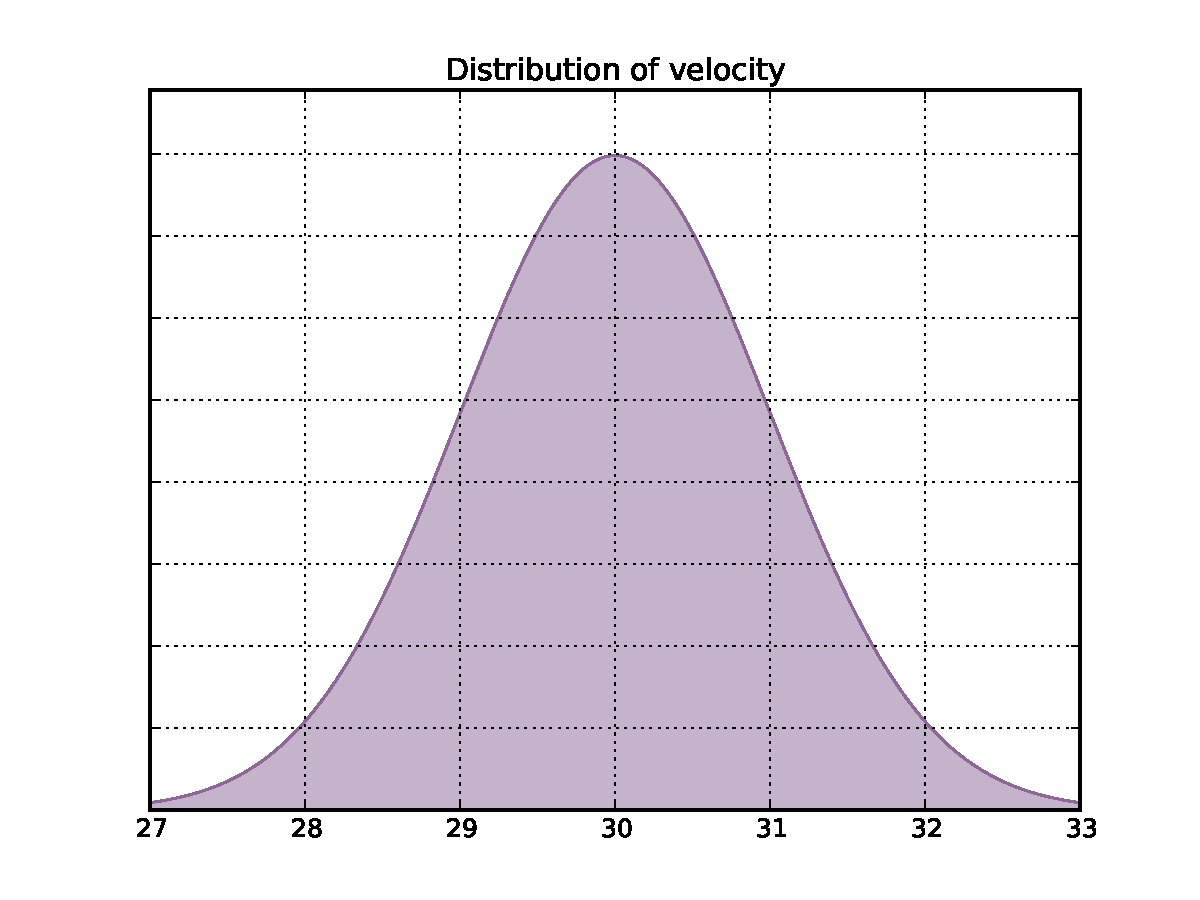
\includegraphics[width=\textwidth]{images/velocity-distribution.pdf}
    \end{figure}
\end{columns}

\begin{columns}<2->
    \column{.5\textwidth}

\begin{lstlisting}
>>> P(v > 31)
\end{lstlisting}

    \column{.5\textwidth}

    $$ - \frac{1}{2} \operatorname{erf}{\left (\frac{1}{2} \sqrt{2} \right )} 
       + \frac{1}{2} == 0.1586...$$

\end{columns}

\end{frame}

\begin{frame}{Graph with Random Expressions}
    Random inputs cause other random expressions
    \begin{figure}
        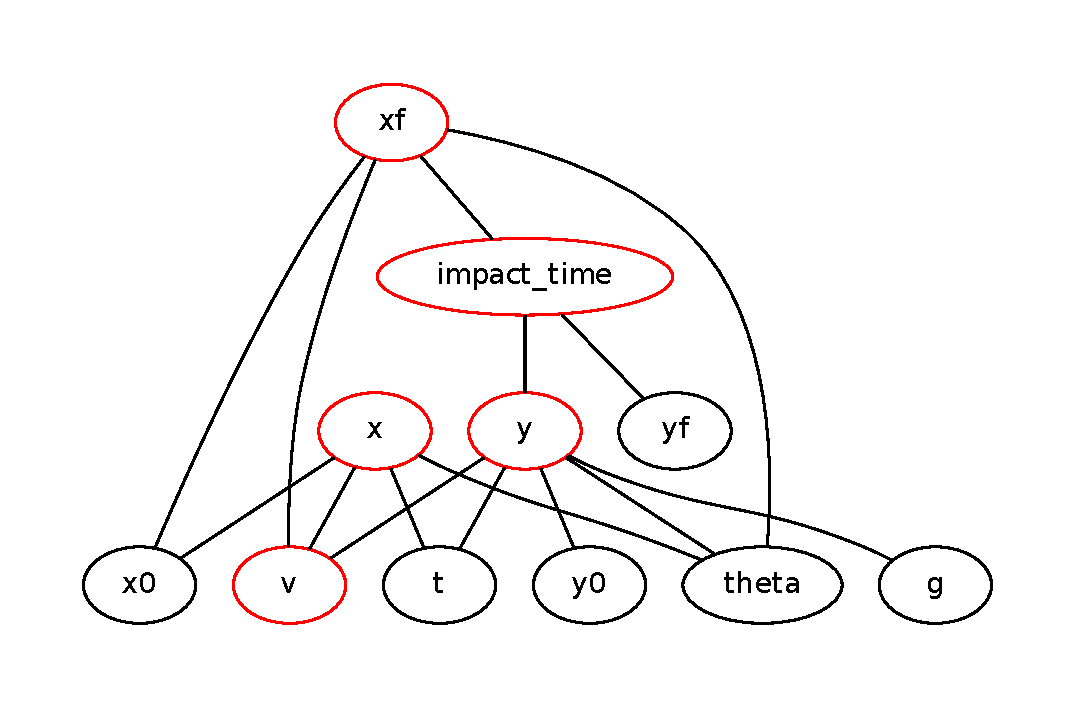
\includegraphics[width=\textwidth]{images/uncertain-dag.pdf}
    \end{figure}

\end{frame}

\begin{frame}[semiverbatim, fragile]{Querying Random Expressions}
    \begin{columns}
        \column{.5\textwidth}

\begin{lstlisting}
a,b = symbols('a,b')
density(x)(a) * density(y)(b)
\end{lstlisting}

        \column{.5\textwidth}
        $$
        \frac{e^{- \frac{a^{2}}{t^{2}}} e^{- \frac{\left(b + 5
            t^{2}\right)^{2}}{t^{2}}} e^{30 \frac{\sqrt{2} a}{t}} e^{30
        \frac{\sqrt{2} \left(b + 5 t^{2}\right)}{t}}}{\pi t^{2} e^{900}}
        $$

    \end{columns}
    \begin{columns}
        \column{.5\textwidth}
\begin{lstlisting}
plot(P(y > yf), (t, 2.7, 3.4))
\end{lstlisting}
        \column{.5\textwidth}
            \begin{figure}
                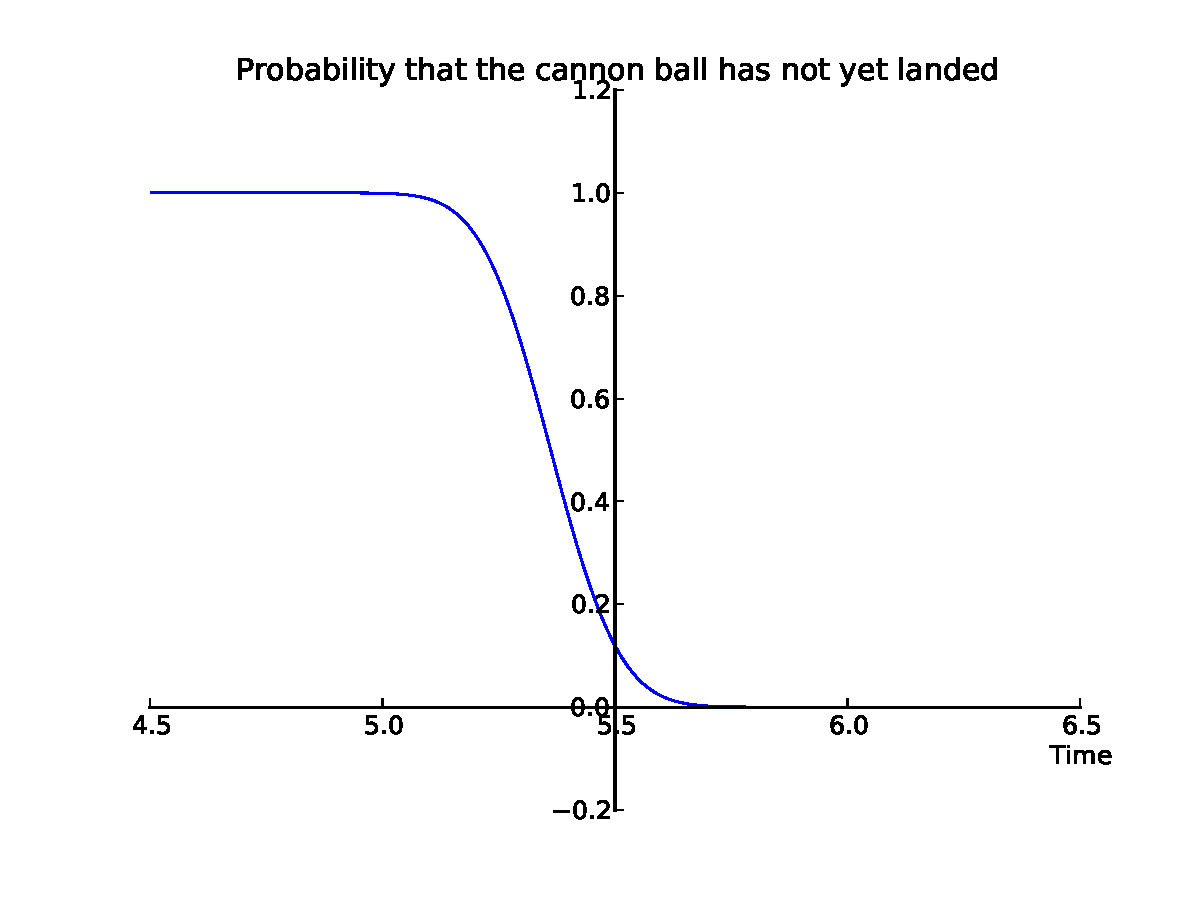
\includegraphics[width=\textwidth]{images/impact.pdf}
            \end{figure}
    \end{columns}
    
    \begin{columns}
        \column{.5\textwidth}
\begin{lstlisting}
E(impact_time)
\end{lstlisting}
        \column{.5\textwidth}
        $$\int_{-\infty}^{\infty} \frac{\left(v + \sqrt{v^{2} + 1200}\right)
        e^{- \frac{1}{2} \left(v -30\right)^{2}}}{20 \sqrt{\pi}}\, dv
        $$
    \end{columns}

\end{frame}

\section{Multi-Compilation}
\subsection{I}

\begin{frame}[semiverbatim]{Random and Computational expressions}
    SymPy.stats does two things
    \begin{enumerate*}
        \item Models uncertain systems
        \item Reduces uncertain expressions to computational ones
    \end{enumerate*}
    Functions P, E, sample, density, variance ::\\ \indent Random Expression $\rightarrow$ Computational Expression

    $P(v > 31) 
    \rightarrow 
    \int_{31}^{\infty} \frac{\sqrt{2} e^{- \frac{1}{2} \left( z - 30\right)^{2}}} {2 \sqrt{\pi}}\, dz
    \rightarrow
    - \frac{1}{2} \operatorname{erf}{\left (\frac{1}{2} \sqrt{2} \right )} + \frac{1}{2}$

    $\textrm{E(impact time)}
    \rightarrow
    \int_{-\infty}^{\infty} \frac{\left(v + \sqrt{v^{2} + 1200}\right) e^{-
    \frac{1}{2} \left(v -30\right)^{2}}}{20 \sqrt{\pi}}\, dv
    \rightarrow
    ?$

    \uncover<2-3>
    {
        But there are other ways to compute integrals
        \begin{enumerate*}
            \item scipy.integrate.quad (uses FORTRAN library)
            \item Monte Carlo \uncover<3>{(\textit{E(impact time, numsamples=10000)})}
            \item Code Generation
        \end{enumerate*}
    }
\end{frame}

\begin{frame}{Other kinds of expressions}
    \begin{table}
        \begin{tabular}{| l | l |}
           \hline
           RV Type                      &  Computational Type  \\
           \hline\hline
           Continuous                   &   SymPy Integral     \\
           \hline
           Discrete - Finite (dice)     &   Python iterators / generators \\ 
           \hline
           Discrete - Infinite (Poisson)&  SymPy Summation              \\
           \hline
           Multivariate Normal          &   SymPy Matrix Expression      \\
           \hline
       \end{tabular}
   \end{table}
\end{frame}

\begin{frame}[semiverbatim, fragile]{Kalman Filter}
\begin{lstlisting}
mu = MatrixSymbol('mu', n, 1) # n by 1 mean vector
Sigma = MatrixSymbol('Sigma', n, n) # covariance matrix
X = MVNormal('X', mu, Sigma) 

H = MatrixSymbol('H', k, n) # An observation operator
data = MatrixSymbol('data', k, 1)

R = MatrixSymbol('R', k, k) # covariance matrix for noise
noise = MVNormal('eta', ZeroMatrix(k, 1), R)

# Conditional density of X given  HX+noise==data
density(X , Eq(H*X+noise, data)  ) 
\end{lstlisting}

\vspace{-30pt}
$$\left[\begin{smallmatrix}\mathbb{I} && \bold{0}\end{smallmatrix}\right] \left(\left[\begin{smallmatrix}\Sigma && \bold{0}\\\bold{0} && R\end{smallmatrix}\right] \left[\begin{smallmatrix}H^T\\\mathbb{I}\end{smallmatrix}\right] \left(\left[\begin{smallmatrix}H && \mathbb{I}\end{smallmatrix}\right] \left[\begin{smallmatrix}\Sigma && \bold{0}\\\bold{0} && R\end{smallmatrix}\right] \left[\begin{smallmatrix}H^T\\\mathbb{I}\end{smallmatrix}\right]\right)^{-1} \left( \left[\begin{smallmatrix}H && \mathbb{I}\end{smallmatrix}\right] \left[\begin{smallmatrix}\mu\\\bold{0}\end{smallmatrix}\right] - data\right) + \left[\begin{smallmatrix}\mu\\\bold{0}\end{smallmatrix}\right]\right)$$

\vspace{-15pt}
$$\left[\begin{smallmatrix}\mathbb{I} && \bold{0}\end{smallmatrix}\right] \left(\mathbb{I} - \left[\begin{smallmatrix}\Sigma && \bold{0}\\\bold{0} && R\end{smallmatrix}\right] \left[\begin{smallmatrix}H^T\\\mathbb{I}\end{smallmatrix}\right] \left(\left[\begin{smallmatrix}H && \mathbb{I}\end{smallmatrix}\right] \left[\begin{smallmatrix}\Sigma && \bold{0}\\\bold{0} && R\end{smallmatrix}\right] \left[\begin{smallmatrix}H^T\\\mathbb{I}\end{smallmatrix}\right]\right)^{-1} \left[\begin{smallmatrix}H && \mathbb{I}\end{smallmatrix}\right]\right) \left[\begin{smallmatrix}\Sigma && \bold{0}\\\bold{0} && R\end{smallmatrix}\right] \left[\begin{smallmatrix}\mathbb{I}\\\bold{0}\end{smallmatrix}\right]$$

$$\begin{smallmatrix}\mu + \Sigma H^T \left(R + H \Sigma H^T\right)^{-1} \left(  H \mu - data\right)\end{smallmatrix}$$
$$\begin{smallmatrix}\left(\mathbb{I} - \Sigma H^T \left(R + H \Sigma H^T\right)^{-1} H\right) \Sigma\end{smallmatrix}$$

\end{frame}

\begin{frame}{Scientific Computing Technology Stack}

        \begin{figure}
            \includegraphics<1>[height=.8\textheight]{images/stack_empty.pdf}
            \includegraphics<2>[height=.8\textheight]{images/stack_full.pdf}
        \end{figure}

\end{frame}

\section{Conclusion}
\subsection{I}
\begin{frame}{End}

    \begin{centering}
        This work was a Google Summer of Code project. 

        Contributors: Raoul Bourquin, Nathan Alison

        GSoC Mentor: Andy Terrel

        SymPy: \url{http://github.com/sympy/sympy}


        me: Matthew Rocklin
        \url{http://matthewrocklin.com}
        \url{http://github.com/mrocklin}

    \end{centering}
\end{frame}

\end{document}
